\documentclass{standalone}
\usepackage{tikz}
\usetikzlibrary{patterns}
\begin{document}
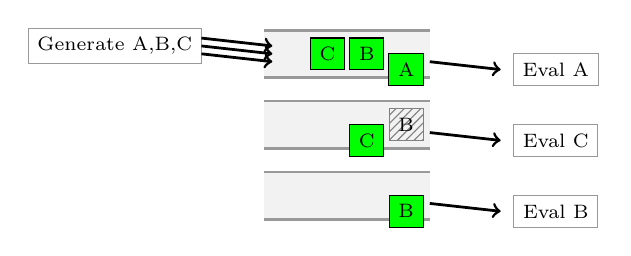
\begin{tikzpicture}
\fill[fill=none] (-3.1,0) rectangle (4.2,0);
\begin{scope}[shift={(0,-0.1)}]
   \draw[fill=black!5,draw=none] (-0.1,-0.3) rectangle (2.0,0.3);
   \draw[line width=1pt,color=black!40] (-0.1,-0.3) -- (2.0,-0.3);
   \draw[line width=1pt,color=black!40] (-0.1, 0.3) -- (2.0, 0.3);
   \node[rectangle,fill=green,draw=black] at (0.7,  0.0) {\scriptsize\centering C};
   \node[rectangle,fill=green,draw=black] at (1.2,  0.0) {\scriptsize\centering B};
   \node[rectangle,fill=green,draw=black] at (1.7, -0.2) {\scriptsize\centering A};
   \node[rectangle,draw=black!40] at (-2.0, 0.1) {\scriptsize\centering Generate A,B,C};
   \draw[line width=1pt,->] (-0.9,0.2) -- (0,0.1);
   \draw[line width=1pt,->] (-0.9,0.1) -- (0,0.0);
   \draw[line width=1pt,->] (-0.9,0.0) -- (0,-0.1);
   \draw[line width=1pt,->] (2.0,-0.1) -- (2.9,-0.2);
   \node[rectangle,draw=black!40] at (3.6, -0.2) {\scriptsize\centering Eval A};
\end{scope}
\begin{scope}[shift={(0,-1.0)}]
   \draw[fill=black!5,draw=none] (-0.1,-0.3) rectangle (2.0,0.3);
   \draw[line width=1pt,color=black!40] (-0.1,-0.3) -- (2.0,-0.3);
   \draw[line width=1pt,color=black!40] (-0.1, 0.3) -- (2.0, 0.3);
   \node[rectangle,fill=green,draw=black] at (1.2, -0.2) {\scriptsize\centering C};
   \node[pattern=north east lines, pattern color=black!50, draw=black!50] at (1.7,  0.0) {\scriptsize\centering B};
   \draw[line width=1pt,->] (2.0,-0.1) -- (2.9,-0.2);
   \node[rectangle,draw=black!40] at (3.6, -0.2) {\scriptsize\centering Eval C};
\end{scope}
\begin{scope}[shift={(0,-1.9)}]
   \draw[fill=black!5,draw=none] (-0.1,-0.3) rectangle (2.0,0.3);
   \draw[line width=1pt,color=black!40] (-0.1,-0.3) -- (2.0,-0.3);
   \draw[line width=1pt,color=black!40] (-0.1, 0.3) -- (2.0, 0.3);
   \node[rectangle,fill=green,draw=black] at (1.7, -0.2) {\scriptsize\centering B};
   \draw[line width=1pt,->] (2.0,-0.1) -- (2.9,-0.2);
   \node[rectangle,draw=black!40] at (3.6, -0.2) {\scriptsize\centering Eval B};
\end{scope}
\end{tikzpicture}%
\end{document}
